\chapter{TLM background theory}
\label{secTLMtheory}
The method that is used to enable interaction between dynamic models in the composite model simulation is \emph{transmission line modelling} (TLM)~\cite{Johns-80}~\cite{KrusModMech-99}~\cite{KrusDistrSim}~\cite{Cogan-06}.
TLM uses physically motivated time delays to separate the components in time and enable efficient co-simulation. 
Only TLM connections between two external interfaces are currently supported by the composite model simulation environment because the TLM method gives numerical stability.


The TLM (\emph{Transmission Line Modeling}) method, also called Bilateral Delay Line Method \cite{Johns-80}, exploites the fact that all physical interactions in nature have finite propagation speed.
\begin{figure}
\begin{center}
   {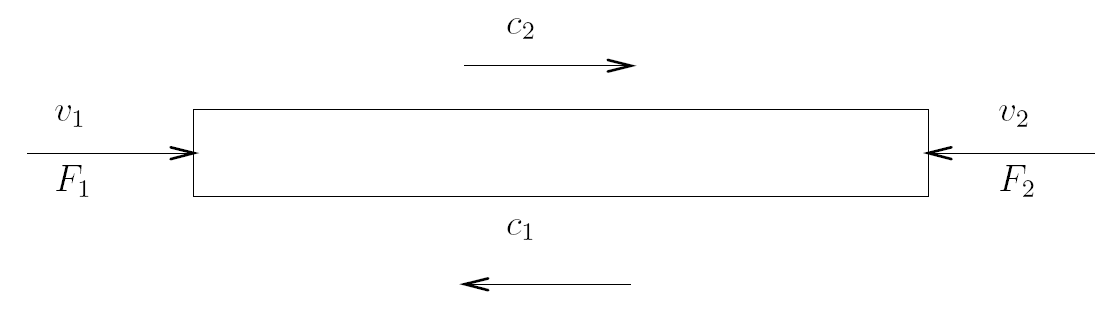
\includegraphics[width=9cm]{figs/TLMline.png}}
\caption{Delay line with the passing wave variables $c_1$ and $c_2$
and velocity variables $v_1$ and $v_2$.}
\end{center}
\label{figTLMline}
\end{figure}

A basic one-dimensional transmission line is shown in Figure \ref{figTLMline}.
For the mechanical case the line is basically an ideal elastic medium with force waves $c_1$ and $c_2$ going between its ends. 
The input disturbances are velocities $v_1$ and $v_2$ and the forces from the transmission line $F_1$ and $F_2$.

Note that the springs in our implementation are assumed to be isotropic.
That is no cross-term waves are generated when working in 2D and 3D. 
See \cite{KrusModMech-99} for further discussions.

If the line delay is set to $T_{TLM}$ and its impedance to $Z_F$ then the govering equations are:
\begin{equation}
\begin{array}{l}
c_1(t) = F_2(t-T_{TLM})+ Z_F \; v_2(t-T_{TLM})\\
c_2(t) = F_1(t-T_{TLM})+ Z_F \; v_1(t-T_{TLM})\\
\\
F_1(t) = Z_F \; v_1(t) + c_1(t) \\
F_2(t) = Z_F \; v_2(t) + c_2(t)
\end{array}
\label{eqTLM}
\end{equation}
The equations show that the two simulation systems are decoupled with the delay time $T_{TLM}$. Simulation framework can utilize this decoupling to enable efficient communications during co-simulation. 

Representing the TLM connection with a simple model of a steel beam, the stiffness coefficient can be computed as (see \cite{KrusModMech-99}):
\begin{equation}
\label{eqKsimple}
k = \frac{E A}{L_0}
\end{equation}
where $E$ is Young's modulus, $A$ is the cross section area and $L_0$ the length of the beam. 

The impedance $Z_F$ has a relation to the spring constant $k$, $Z_F = k T_{TLM}$. 
The impedance factor can then be formulated as a function of the area and length of the steel rod according to
\begin{equation}
\label{eqZFsimple}
Z_F = \frac{E A T_{TLM}}{L_0}
\end{equation}

\begin{figure}
\begin{center}
   {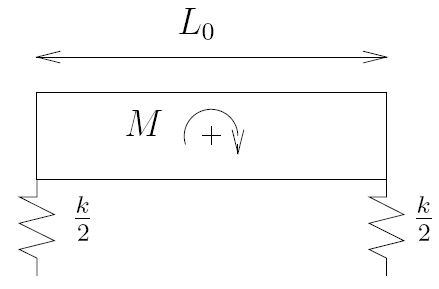
\includegraphics[width=9cm]{figs/RotStiff.png}}
\caption{Estimating the rotational stiffness.}
\end{center}
\label{figRotStiff}
\end{figure}

To get the stiffness and impedance for the rotational degrees of freedom one can use the already computed stiffness $k$. If the arrangement depicted in
Figure \ref{figRotStiff} is assumed, then:
\begin{equation}
k_{\phi} = \frac{M}{\delta_{\phi}} = 2 \frac{ (k/2) \delta_{\phi} (L_0/2)^2}{\delta_{\phi}} = \frac{k L_0^2}{4}
\label{eqKphi}
\end{equation}

and the impedance for the rotation:
\begin{equation}
Z_{FR} = \frac{1}{4}Z_F L_0^2
\end{equation}

The time constant $T_{TLM}$ can be computed using the speed of sound for the medium:
\begin{equation}
\label{eqTtlm}
T_{TLM} = \frac{L_0}{v_{medium}}
\end{equation}

It can be shown that the TLM element also introduces a (\emph{parasitic mass}) that can be viewed to be outside the simulated system \cite{KrusModMech-99}. The total mass for the combined systems must therefore also
include the parasitic mass of the TLM element in order to make, e.g., the energy conservation formulas correct. This mass depends on the impedance factor and the time delay factor
\begin{equation}
\label{eqMtlm}
m_p = Z_F T_{TLM}
\end{equation}

This implies that if the impedance factor $Z_F$  is increased, the parasitic mass will increase if the synchronization delay $T_{TLM}$ is not decreased. 
If the parasitic mass is large it may influence the system behavior and can not be neglected. 
Note, that for the simple beam case when TLM parameters are computed according to Equations \ref{eqZFsimple} and \ref{eqTtlm} the parasitic mass is equivalent to the mass of the beam ($\rho A L0$, where $\rho$ is the material density).

For practical purposes (see \cite{Fritzson+Stahl+Nakhimovski-07}) one can use the parameters of a material cube with an edge given by \emph{characteristic distance} $L_0$. 
Equations \ref{eqKsimple} and \ref{eqKphi} can then be used to compute the translational and rotational stiffnesses:
\begin{equation}
\begin{array}{l}
k = \frac{E L_0 ^2}{L_0} = E L_0 \\
\\
k_{\phi} = \frac{k L_0^2}{4} = \frac{E L_0^3}{4}
\end{array}
\end{equation}

To give a concrete example, let us assume that connection medium is steel and the characteristic length is $L_0 = 0.1$. Steel has  Young's modulus $E = 210 GPa$ and the speed of sound in steel is $v_{steel}=5180 m/s$.
The TLM parameters then can be computed:
\begin{equation}
\begin{array}{l}
T_{TLM} = L_0 / v_{steel} \approx 2*10^{-5} \\
\\
Z_F =  E L_0 T_{TLM} \approx 2 * 10^5 \\
\\
Z_{FR} =  \frac{1}{4}Z_F L_0^2 \approx 500
\end{array}
\end{equation}

Calculations like these give approximate values of the stiffness and the time delay of the TLM element. 
This gives a background for selecting the TLM line delay and impedance parameters.
In cases when required $T_{TLM}$ becomes a limiting factor, while the TLM link stiffness is much higher than the stiffnesses used in the sub-models, a lower stiffness and larger $T_{TLM}$ may be considered.

The elastic medium that is modelled with the TLM element introduces oscillation frequencies (standing waves) given by:
\begin{equation}
\label{eqTspring}
f_{TLM, i} = \frac{i}{2\;T_{TLM}}, \;\; i = 1, 2, 3, ...
\end{equation}

The basic TLM model has no damping which can result in unwanted vibrations during simulation.
In \cite{KrusModMech-99} a low pass filtering of the TLM charateristics is recommended:
\begin{equation}
c_{\ri{filtered}}(t) = c_{\ri{filtered}}(t - T) \; \alpha + c(t) \; (1 - \alpha)
\end{equation}
The filtering is controlled by a damping constant $\alpha$. 
The recommended value according to~ \cite{KrusModMech-99} is $0.2$.

